\documentclass[10pt,a4paper]{amsart}
\usepackage[margin=19mm]{geometry}
\usepackage{amsmath,amssymb,mathtools}
\usepackage[scr=rsfs,cal=euler]{mathalfa}
\usepackage{xfrac}
\usepackage[unicode,hidelinks,bookmarks=false]{hyperref}
\newcommand{\ie}{i.e.\ }
\newcommand{\cf}{cf.\ }
\newcommand{\resp}{respectively\ }
\newcommand{\Subsection}{\subsection}
\providecommand{\nobreakdash}{\nobreak\hbox{-}}
\setlength{\emergencystretch}{2em}
\multlinegap0pt
\usepackage{tikz}
\usepackage{float}
\usepackage{amssymb}
\usepackage{xcolor}
\newtheorem{theorem}{Theorem}
\title{Permutations with a fixed number of occurrences of a pattern: a case generalizing 231}
\author{Michael Waite}
\date{Source: arXiv:2603.21625v2 (CC BY 4.0)}
\begin{document}
\maketitle

\noindent\emph{Source and licence.} Permutations with a fixed number of occurrences of a pattern: a case generalizing 231. Version arXiv:2603.21625v2 (CC BY 4.0), distributed by arXiv under the Creative Commons Attribution 4.0 International licence, http://creativecommons.org/licenses/by/4.0/, as recorded in the arXiv licence metadata for this exact version and shown on the abstract page https://arxiv.org/abs/2603.21625v2. Full licence notice: \texttt{licenses/arxiv-2603.21625-CC-BY-4.0.txt}.\par\smallskip

\noindent\textit{Editorial scope.} Counted unit: the article's theorem theorem (source0.tex lines 218--225). The article's complete original proof of it is delivered with it (source0.tex lines 227--291, one \texttt{proof} environment of 65 lines). No mathematics is written, repaired or re-derived: the statement and the proof are the article's own lines, in the article's own notation, and no retained line is substituted or re-flowed.  No further source-local context is needed: every cross-reference of every retained line resolves inside the two delivered spans.  Nothing was omitted from any retained span, so the package carries no omission record.  No retained line contains a citation, so the wrapper carries no bibliography and no bibliography entry.  The retained lines contain the article's own diagram code, which the wrapper typesets with the standard tikz packages; no image file is delivered and the package declares no asset dependency.  Editorial formatting only, in addition: an AMS \texttt{amsart} preamble that restates the article's own declarations and macros used by the retained lines, namely the environments \texttt{theorem} on separate counters, together with the standard packages those lines need.  The retained environments print in this document as Theorem 1 in order of appearance, whereas the article prints the same items with the numbering of its own full document.  The complete native source of the article as distributed in the arXiv e-print for this exact version is bundled unchanged as \texttt{sources/196963/source0.tex}.
\begin{theorem}
    Let $q$ be a permutation of length $m$ which is indecomposable, and is of the form $q_1 \ominus ... \ominus q_k$ for some $k \geq 2$ where all of the $q_i$ are skew-indecomposable and $q_2, ..., q_{k-1}$ are not $1$. Let $q_1$ be of length $\ell$.  Suppose $r \geq 1$. Then there is an injection
    \[
    \phi: \mathcal{I}_{n-rm-\ell+1, r} \times S_{n - rm - \ell}(q) \hookrightarrow S_{n,r}(q)
    \]
    for $n\geq rm$.

\end{theorem}

\begin{proof}
    Let $p\in S_{n - rm - \ell }(q)$ and let $S \in \mathcal{I}_{n-rm-\ell+1, r}$. Let $s_1, ..., s_{r}$ be the entries in $S$ in increasing order. Replace $p$ by $q_1 \oplus p \in Av_{n - rm}(q)$, so that we can assume that $p$ begins with a copy of $q_1$, and replace each $s_i$ by $s_i + \ell$.
    
    Our main idea is that we will insert a copy of $q$ in certain blocks of consecutive values at each of the positions $s_1, ..., s_{r}$ in $p$, and we will choose these blocks of values in such a way as to not create extra $q$ patterns.

    Now we will define these blocks of values. Let $B_1$ consist of $q_1$ and all of the values of $q_2$ except for the smallest value. For $2\leq i \leq k-2$, let $B_i$ be the set of values consisting of the smallest value of $q_i$ and all of the values of $q_{i+1}$ except for the smallest value. Let $B_{k-1}$ be the set of values consisting of the smallest value of $q_{k-1}$ and all of $q_k$. For $1 \leq i \leq k$ let $b_i = |B_i|$. 
    
    % Now $\cup_{i=1}^{k-1} B_i = [m]$ and no $B_i$ contains all of the values of $q_i$ $q_i$, except for $B_1$ which contains $q_1$ and $B_{k-1}$ which contains $q_k$.

    Now we will insert copies of $q$ iteratively starting at $s_1$. For $1\leq i \leq k-1$ let $a_i$ be the largest entry that is the smallest entry of a $q_1 \ominus ... \ominus q_i$ pattern that is entirely to the left of $s_1$. Insert a copy of $q$ in position $s_1$ with the values of $B_i$ in between $a_i$ and the next larger entry.

    Let $L_1$ be the subsequence of entries to the left of $s_1$ with value greater than $a_1$. For $2\leq i \leq k-1$, let $L_i$ be the subsequence of entries to the left of $s_1$ with value greater than $a_i$, and less than or equal to $a_{i-1}$. Let $L_{k}$ be the subsequence of entries to the left of $s_1$ with value less than or equal to $a_{k-1}$. Likewise define $R_1$, ..., $R_k$ for entries to the right of $s_1$.

    \begin{figure}[H]
        \centering
        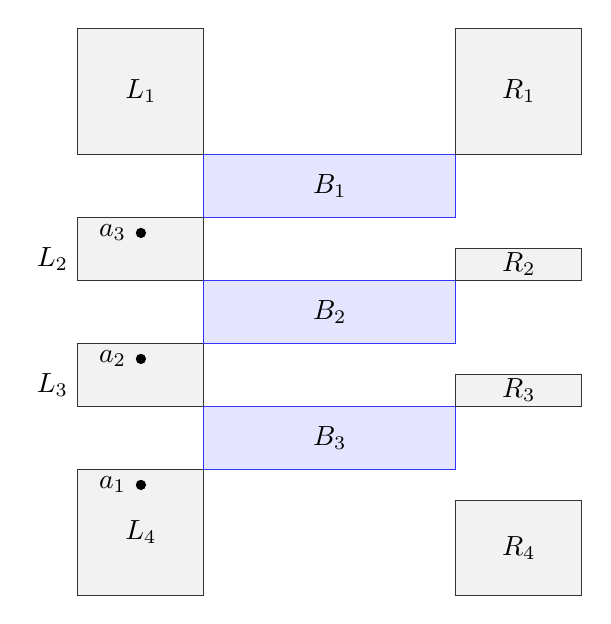
\begin{tikzpicture}[scale = .8, point/.style={circle,draw=black!100,fill=black!100,thick,
                     inner sep=0pt,minimum size=1mm},
                          ]
                          
      \draw[draw = black!80!,fill=gray!10] (0,0) rectangle node[anchor= center]{$L_4$} (2,2);
      \draw[draw = black!80!,fill=gray!10] (0,3) node[anchor= south east]{$L_3$} rectangle  (2,4);
      \draw[draw = black!80!,fill=gray!10] (0,5) node[anchor= south east]{$L_2$}rectangle  (2,6);
      \draw[draw = black!80!,fill=gray!10] (0,7) rectangle node[anchor= center]{$L_1$} (2,9);

      \draw[draw = blue!80!,fill=blue!10] (2,2) rectangle node[anchor= center]{$B_3$} (6,3);
      \draw[draw = blue!80!,fill=blue!10] (2,4) rectangle node[anchor= center]{$B_2$} (6,5);
      \draw[draw = blue!80!,fill=blue!10] (2,6) rectangle node[anchor= center]{$B_1$} (6,7);


     
      \draw[draw = black!80!,fill=gray!10] (6,0) rectangle node[anchor= center]{$R_4$} (8,1.5);
      \draw[draw = black!80!,fill=gray!10] (6,3) rectangle node[anchor= center]{$R_3$} (8,3.5);
      \draw[draw = black!80!,fill=gray!10] (6,5) rectangle node[anchor= center]{$R_2$} (8,5.5);
      \draw[draw = black!80!,fill=gray!10] (6,7) rectangle node[anchor= center]{$R_1$} (8,9) ;

      \node (a1) at (1,1.75) [point] [label=left:$a_1$] {};
      \node (a2) at (1,3.75) [point] [label=left:$a_2$] {};
      \node (a3) at (1,5.75) [point] [label=left:$a_3$] {};
          

        \end{tikzpicture}
        \caption{Insertion of a $q$ pattern at position $s_1$, where $k = 4$}.
        \label{fig:placeholder}
    \end{figure}
    


    For $1\leq i \leq k-1$, by the definition of $a_i$ then the entries contained in $L_1 \cup ... \cup L_i$ cannot contain a $q_1 \ominus ... \ominus q_i$. Because $p$ does not contain any $q$ patterns with entries to the right of $s_1$, then for $2 \leq i \leq k$ the entries contained in $R_i \cup ... \cup R_k$ cannot contain a $q_i \ominus ... \ominus q_k$ pattern.

    Say there were a $q$ pattern with some entries in the $B_i$ blocks and some entries not in the $B_i$ blocks. Let $m$ be minimum so that there are some entries in this $q$ pattern in $B_m$, and $M$ be maximum so that there are some entries in this $q$ pattern in $B_M$. 

    Since $L_1 \cup ... \cup L_m$ cannot contain $q_1 \ominus ... \ominus q_m$, then the $q_m$ in the $q$ pattern must have some entries in $B_m$. Since $R_{M+1} \cup ... \cup R_k$ cannot contain any $q_{M+1} \ominus ... \ominus q_k$ pattern, then the $q_{M+1}$ in the $q$ pattern must have some entries in $B_M$. The possible ways to place a $q_i$ for $m\leq i \leq M+1$ so that not all of the entries are in a $B_j$ for some $j$ now must be either with some entries to the left of $B_m$ and some entries in $B_m$, some entries in $B_m$ and some entries in $B_{m+1}$, ..., some entries in $B_{M-1}$ and some entries in $B_M$, or some entries in $B_M$ and some entries to the right of $B_M$, or if $m = 1$ then all of $q_m$ may be entirely in $B_m$ or if $M = k$ then all of $q_M$ may be entirely in $B_M$. There are $M-m + 2$ of these spots and $M-m + 1$ blocks $q_m, ... q_{M+1}$, so it must be the case that either $q_m$ has some entries to the left of $B_m$ or $q_{M+1}$ has some entries to the right of $B_M$, or that $m=1$ and $M=k$ and all of $q_m$ is in $B_m$ and all of $q_M$ is in $B_M$. The latter case can be discarded since in this case $q$ will have no entries outside of the $B_i$ blocks which is a contradiction. Specifying to the former case, since $q_m$ and $q_{M+1}$ are skew indecomposable then either $q_m$ has some entries below and to the left of $B_m$ or $q_{M+1}$ has some entries above and to the right of $B_M$ .
    
    If $q_{M+1}$ has some entries above and to the right of $B_M$, then all of $q_1 ... q_M$ must be in $B_m \cup ... \cup B_{M-1} \cup L_1 \cup ...\cup L_m$. Since $L_1 \cup ...\cup  L_m$ cannot contain $q_1 \ominus ... \ominus q_m$, then $q_m$ must have some entries in $B_m$. So $B_m \cup ... \cup B_{M-1}$ must contain some entries of $q_m$ and $q_{M+1}$ and all of the entries of $q_{m+1}, ..., q_M$. Since there are $M-m$ blocks $B_m ... B_{M-1}$ and $M-m$ blocks of entries $q_{m+1}, ... q_M$, then it must be that some $q_i$ is entirely contained in some $B_j$, which is a contradiction.

    The case where $q_m$ has some entries below and to the left of $B_m$ results in a similar contradiction.
    % So this $q_{M+1}$ has no entries above and to the right of $B_M$.
    

    % In order for the $q$ pattern we have inserted to create any extra $q$ patterns, there would have to either be a $q_1$ pattern in $L_1$ or a $q_2$ pattern in $R_2$. But neither of these is possible, so there are no extra copies of $q$.
    
    Notice now that in the above argument we only required that the entries after $s_1$ do not contain entries in a $q$ pattern. This condition is now satisfied for $s_2$, so we can repeat the above argument for $s_2$, and again for $s_3, ..., s_{r}$, until we get a permutation in $S_{n,r}(q)$ which we call $\phi(p)$.

    To see that $\phi$ is injective, given $\phi(p)$ we can remove all of the entries that participate in $q$ patterns except for the leftmost $q$ pattern, and store the $r$ positions where each consecutive $q$ pattern was inserted to obtain $S$. Finally we can remove the leftmost $q_1$ pattern from the permutation to obtain $p$.
\end{proof}

\end{document}
